\chapter{méthodes (MIC 2010)}

J'ai utilisé la base de donnée présentée dans la partie\ref{lab:bdd} pour évaluer les performances des techniques de correction du mouvement respiratoire présentés dans le chapitre \ref{lab:corrMvt}. 

Les techniques de correction du mouvement implémentées sont les suivantes :

\begin{enumerate}
 \item Correction pendant la reconstruction par modification de la matrice système (voir section \ref{lab:corrMatSyst})
 \item Correction post-reconstruction par recalage des images prises à différents instants du cycle (voir section \ref{lab:corrPostRecon})
\end{enumerate}

Elles sont comparées avec les images non Corrigées et des images statiques (qui représentent une correction parfaite).

Dans le cas présent, l'objectif est de d'évaluer les performances des techniques de correction du mouvement sur la détection des lésions de faible contraste/faible diamètre. Pour cela, je vais comparer les performances d'un système de détection automatique sur les différents types d'images.

\section{Système CAD}

Le système CAD utilise des informations fréquentielles obtenue par décomposition des images en ondelettes Biorthogonale 4.4. Ces données sont utilisées par le système de classification basé sur un SVM travaillant voxel par voxel. Une étape de réduction des faux positifs est ajoutée par la suite.

\subsection{Classifications}

\begin{enumerate}
 \item Décomposition des images en ondelettes : Pour chaque voxel de l'image d'origine, on obtient entre 8 et 32 coefficients, qui correspondent au vecteur de caractéristiques utilisés par le classifieur
 \item Extraction de la base d'apprentissage : Les coefficients des centres de toutes les tumeurs sont extraites des volumes décomposés, et vont former la base d'apprentissage H1 (positifs). Un certain nombre de voxels sont tirés aléatoirement dans chaque images et leur coefficients sont ajoutés à la base H0 (négatifs).
 \item Apprentissage : Le classifieur SVM est entraîné sur cette base d'apprentissage pour générer le modèle qui sera utilsé pour le test.
 \item Tests : Le SVM entraîné est utilisé pour classer chaque voxel contenu dans les organes à evaluer (poumon et foie).
 \item Réduction des Faux-positifs : Les points sont aggrégés en composantes connexes (connexité 27 en 3 dimensions). Chaque aggrégat est testé pour déterminer si il odit être considéré comme un faux positif ou un vrai positif.
\end{enumerate}

\section{Optimisation des paramètres du classifieur}
\label{lab:optim}

Les différentes étapes de l'évaluation des performances nécéssitent la fixation d'un grand nombre de paramètres. Tous ceux qui correspondent à l'étape de classification sont adaptés à la modalité à évaluer, tandis que ceux relatifs au processus dans son ensemble sont fixés une seule fois.

\subsection{Paramètres à optimiser pour chaque modalité}

\begin{description}
 \item[C] Le terme de pénalisation des exemples mal classés par le classifieur
 \item[gamma] La largeur de bande du RBF du noyau du classifieur
 \item[j] Le niveau de décomposition des images 
\end{description}

J'ai effectué une recherche exaustive par grille avec les paramètres suivants :

\begin{description}
 \item [C] de 1 à 10000 en 15 pas logarithmique
 \item [gamma] de 0.0001 à 1 en 15 pas logarithmique
 \item [j] de 1 à 4, soit de 8 à 32 caractéristiques
\end{description}

L'optimisation a été réalisée à l'aide du logiciel rapid-i~\cite{mierswa2006} pour chaque modalité. Les indicateur de performance (Sensibilité, SPécificité, Précision) sont obtenues en réalisant une cross-validation à 5 étapes sur l'ensemble de la base d'apprentissage. Le triplet de paramètre retenu est celui qui maximise la sensibilité.

J'ai joint pour chaque modalité le front de pareto positionnant chaque triplet dans un espace à deux dimensions (`Sensibilité', 'Spécificité'). Cela permet de vérifier que le crière choisit (maximisation de la sensibilité) ne se fait pas trop au détriment de la spécificité.

% 
% Paramètres retenus :
% 
% \begin{table}[h!]
% 	\label{lab:resOptim}
% 	\centering
% 	\begin{tabular}{|c|c|c|c|}
% 		\hline
% 				& C	& gamma		& j\\
% 		\hline
% 		ET-Static	& 10000 & $1 \times 10^{-4}$	& 3\\
% 		\hline
% 		ET-LOR		& 631	& $2.5 \times 10^{-4}$	& 3\\
% 		\hline
% 		ET-IM		& 3981	& $1 \times 10^{-4}$	& 4\\
% 		\hline
% 		ET-NoCorr	& 100	& $6.31 \times 10^{-4}$	& 3\\
% 		\hline
% 	\end{tabular}
% 	\caption{Paramètres optimisé pour l'entraînement du système CAD}
% \end{table}

\section{Réduction des faux positifs}

\subsection{Technique simple : Critère basés sur l'intersection}

Les points classés positifs sont regroupés en amas de points connexes (connexité 27 en 3D). Il y a un ensemble de règles qui vont déterminer si un amas intersectant une lésions représente un vrai positif. Soit $L$ l'ensemble des points de la lésion, $A$ les points correspondant à l'amas candidat.

\begin{description}
 \item[$card( L \cap A ) > \alpha \times card( L )$] avec $\alpha$ fixé à 0.05 qui fixe la proportion minimale de la tumeur qui doit être présente dans l'amas. Elle permet d'éviter les amas qui intersecteraient la tumeur par accident.
 \item[$card( L \cap A ) > \beta \times card( A )$]  avec $\beta$ fixé à 0.20 limite l'étendue de l'amas en dehors de la tumeur.
\end{description}

\subsection{Technique étendue : Basés intersection et étendue spatiale}

Ce second algorithme est basé sur le premier auquel il ajoute deux critères qui limitent la forme de l'amas.

Il faut définir l'étendue maximale de l'amas selon les différentes dimensions $d$ : $\delta_d$. Soit $\delta_d(A) = max_d(A) - min_d(A)$ avec $max_a$ la position la plus 

\begin{description}
 \item[Volume englobant] Le volume du plus petit rectangle englobant l'amas
 \item[]
\end{description}

$max \left( \frac{\delta_x}{\delta_y}, \frac{\delta_x}{\delta_z}, \frac{\delta_y}{\delta_x}, \frac{\delta_y}{\delta_z}, \frac{\delta_z}{\delta_x}, \frac{\delta_z}{\delta_y} \right)$


Une seconde étape a été ajoutée pour limiter l'étalement de certains amas :

Limitations de volume englobant + Limitation des différences d'étendue des amas entres les 3 dimensions.


\chapter{Analyse des résultats}

% Je comparerais les performances du système CAD selon les deux techniques de réduction des faux positifs ainsi que sur un CAD optimisé/avec des valeurs par défaut.

% \section{Comparaison des résultats}
% 
% Les performances sont évaluées en deux temps : Tout d'abord, je recherche le seuil du classifieur qui engendre 30 Faux positifs (+/- 1). Cela permet de comparer les performances en LLF (analogue à la sensibilité) du classifieur pour un taux de faux positifs donné. Ensuite, je compare les courbres Free-ROC pour voir le comportement des classifieurs sur l'ensemble des NLF (nombre moyen de faux positifs par image).
% 
% 
% \subsection{Classifieur non optimisé pour le poumon}
% 
% Résultats fig.\ref{lab:resPerfNonOpt}. Il faut rappeler qu'il y a en tout 173 lésions dans les images simulées, ce qui amène à un score maximal de 56\% obtenu pour Les image non corrigées.
% 
% \begin{table}[h!]
% 
% \begin{center}\textbf{Classifieur non optimisé} \end{center}
% 
%  Avec réduction des faux positifs simple :
% 
% \begin{center} 
% \begin{tabular}{|c|c|c|c|}
%   \hline
%   Modalité	& Seuil	& NLF	& Nombre de VP \\
%   \hline  
%   ET-Static	& -0.6	& 29.5		& \textbf{72} \\
%   \hline
%   ET-LOR	& -0.94	& 30.5		& 59 \\
%   \hline
%   ET-IM		& -0.69	& 30.6		& 65 \\
%   \hline
%   NoCorr	& 1.3	& 30.5		& 63 \\
%   \hline
%  \end{tabular}
%  \end{center}
% 
% \vspace{0.5cm}
%  Avec réduction des faux positifs étendue :
%  \begin{center}
%  \begin{tabular}{|c|c|c|c|}
%   \hline
%   Modalité	& Seuil	& NLF	& Nombre de VP \\
%   \hline  
%   ET-Static	& 0.89	& 29.8		& 69 \\
%   \hline
%   ET-LOR	& 0.04	& 26.7		& 68 \\
%   \hline
%   ET-IM		& 0.37	& 29.6		& 82 \\
%   \hline
%   NoCorr	& -0.23	& 29.5		& \textbf{97} \\
%   \hline
%  \end{tabular}
%  \end{center}
% 
%  \caption{Nombre de Vrai Positifs (VP) obtenu par un CAD non optimisé en acceptant 30 Faux positifs par image (NLF), selon les deux techniques de réduction des faux positifs}
%  \label{lab:resPerfNonOpt}
% 
% \end{table}
% 
% 
% \subsection{Classifieur optimisé pour le poumon}
% 
% Résultats présentés \ref{lab:resPerfOpt}. Il faut rappeler qu'il y a en tout 173 lésions dans les images simulées, ce qui amène à un score maximal de 56\% obtenu pour corrigées par ET-IM.
% 
% \begin{table}[h!]
%  
% 
% \begin{center}\textbf{Classifieur optimisé} \end{center}
% 
%  Avec réduction des faux positifs simple :
%  \begin{center}
%  \begin{tabular}{|c|c|c|c|}
%   \hline
%   Modalité	& Seuil	& NLF	& Nombre de VP \\
%   \hline  
%   ET-Static	& -1.9	& 30.3		& 14 \\
%   \hline
%   ET-LOR	& -1.9	& 29.3		& 3 \\
%   \hline
%   ET-IM		& -1.4	& 30.5		& \textbf{38} \\
%   \hline
%   NoCorr	& -1.5	& 30.3		& 19 \\
%   \hline
%  \end{tabular}
%  \end{center}
% 
% \vspace{0.5cm}
%  Avec réduction des faux positifs étendue :
% 
%  \begin{center}
%  \begin{tabular}{|c|c|c|c|}
%   \hline
%   Modalité	& Seuil	& NLF	& Nombre de VP \\
%   \hline  
%   ET-Static	& 1.5	& 30		& 70 \\
%   \hline
%   ET-LOR	& 0.9	& 30.9		& 76 \\
%   \hline
%   ET-IM		& 0.0	& 29.6		& \textbf{98} \\
%   \hline
%   NoCorr	& -0.3	& 29.8		& 93 \\
%   \hline
%  \end{tabular}
%  \end{center}
% 
%  \caption{Nombre de Vrai Positifs (VP) obtenu par un CAD non optimisé en acceptant 30 Faux positifs par image (NLF), selon les deux techniques de réduction des faux positifs}
%  \label{lab:resPerfOpt}
% \end{table}


\section{Tests de différents paramètres}

Tests de 3 types de paramètres : 

\begin{description}
 \item[Normalisation :] Les données sont normalisées de manière à ce que la moyenne et l'écart-type de chaque caractéristique soit de 1 ($(\mu, \sigma)=(1,1)$) (mean), ou que l'ensemble des valeurs soit comprises entre -1 et +1 (range).
 \item[Nombre de points de la base d'apprentissage :] Le nombre de points extraits de chaque image pour alimenter la base d'exemples normaux peut avoir une influence sur les résultats. Deux valeurs sont testées. 200 pts/im. (soit 3000 pts. négatifs) et 1000 pts/im. (soit 15000 pts. négatifs)
 \item[positions des points extraits :] Une érosion est réalisée sur les images avant d'extraire les points négatifs. Cele permet de retirer les points de la base d'apprentissage qui pourraient poser des problèmes 
\end{description}

\begin{figure}[h!]
\label{fig:paretoParams1}
\begin{center}
 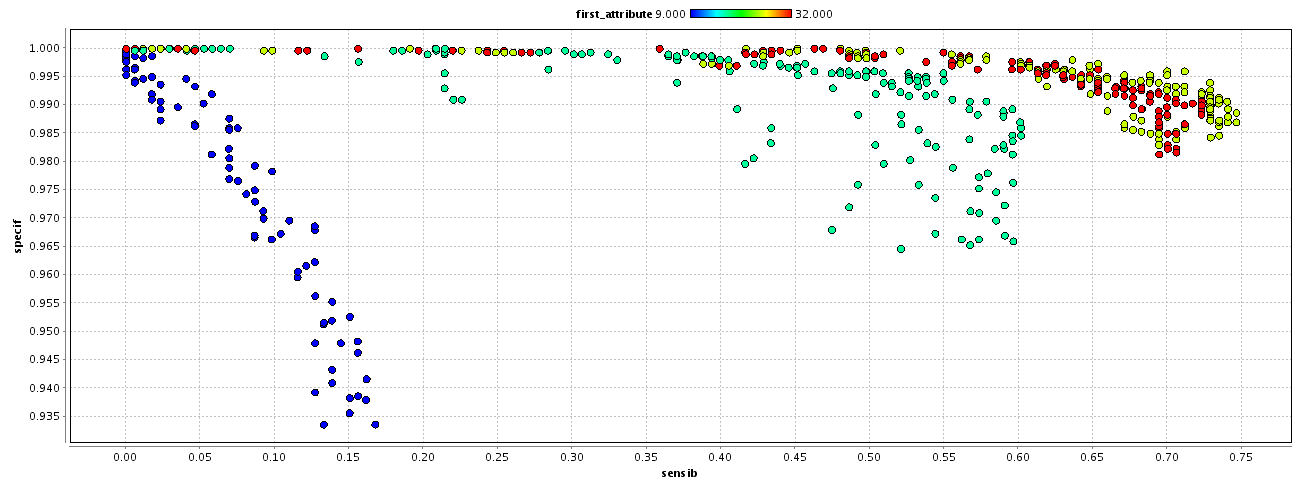
\includegraphics[width=14cm]{images/pareto_param_200.png}

{\small a) Base Témoin}
\vspace{0.5cm}

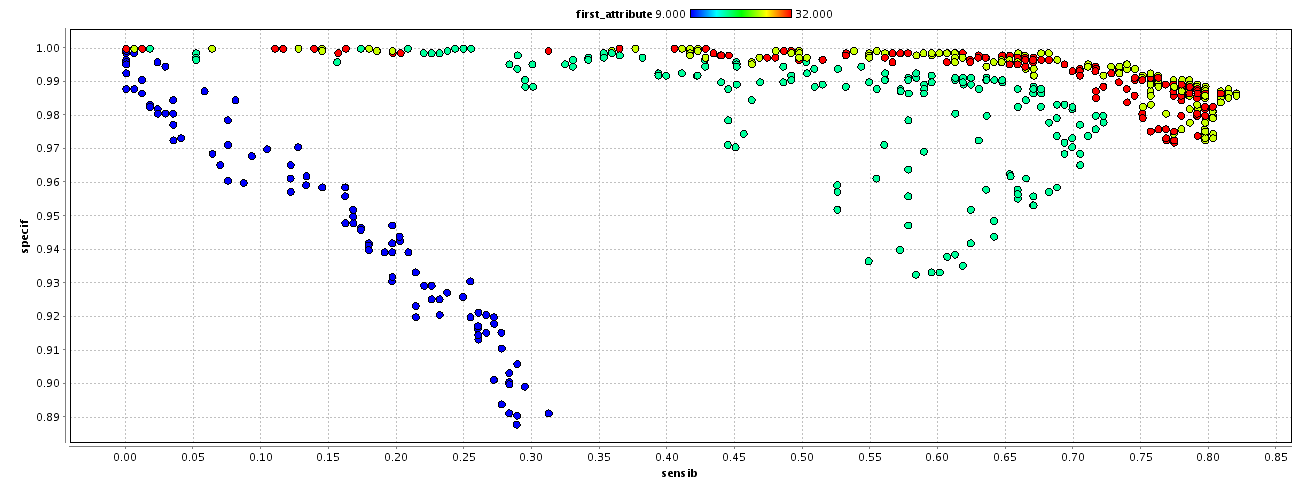
\includegraphics[width=14cm]{images/pareto_param_100.png}

{\small b) Base appauvrie}


 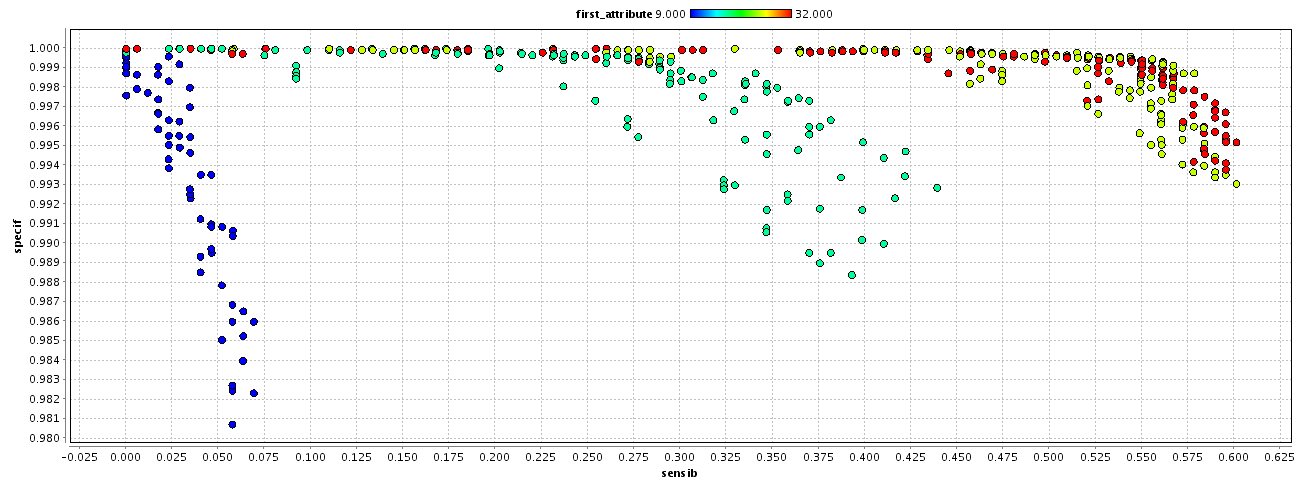
\includegraphics[width=14cm]{images/pareto_param_1000.png}
 
{\small c) Base enrichie}



\end{center}
 \caption{Fronts de pareto des résultats de la recherche des meilleurs paramètres du classifieur (1/2). Pour chaque triplet de paramètres (C, $\gamma$, j), la sensibilité et la spécificité sont reportées sur le graphique. Le code couleur correspond à la valeur de j. En a), la base témoin, avec 200 points négatifs par image et une normalisation mean, en b) la base appauvrie avec 100 points négatifs par image et une normalisation mean, et en c) la base enrichie avec 1000 points négatifs par image et une normalisation mean.}
\end{figure}



\begin{figure}[h!]
\label{fig:paretoParams2}
\begin{center}

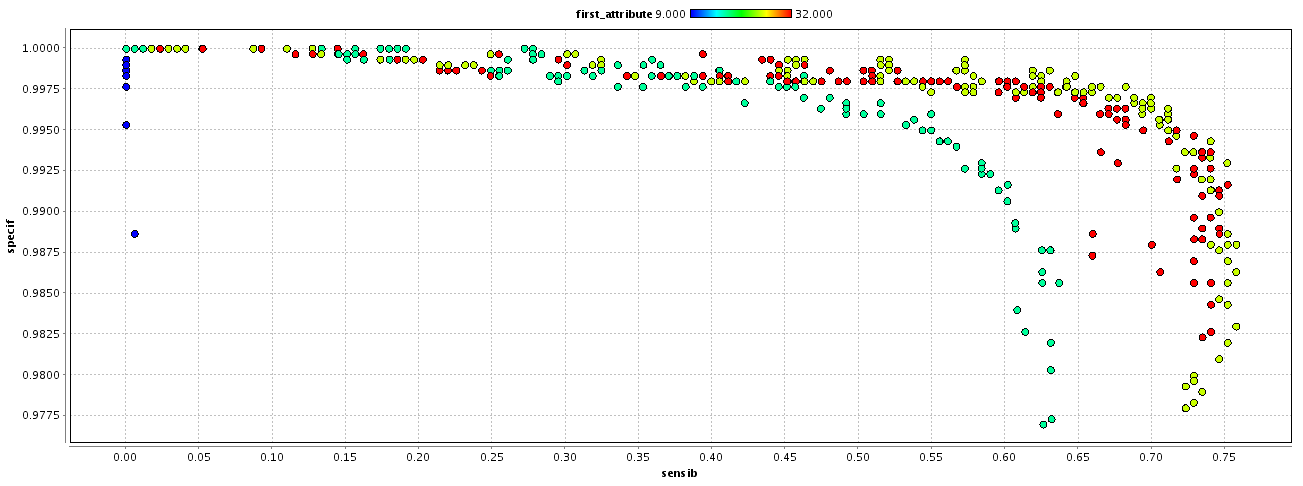
\includegraphics[width=14cm]{images/pareto_param_range.png}

{\small d) Base Normalisée -1/+1}

\vspace{0.5cm}

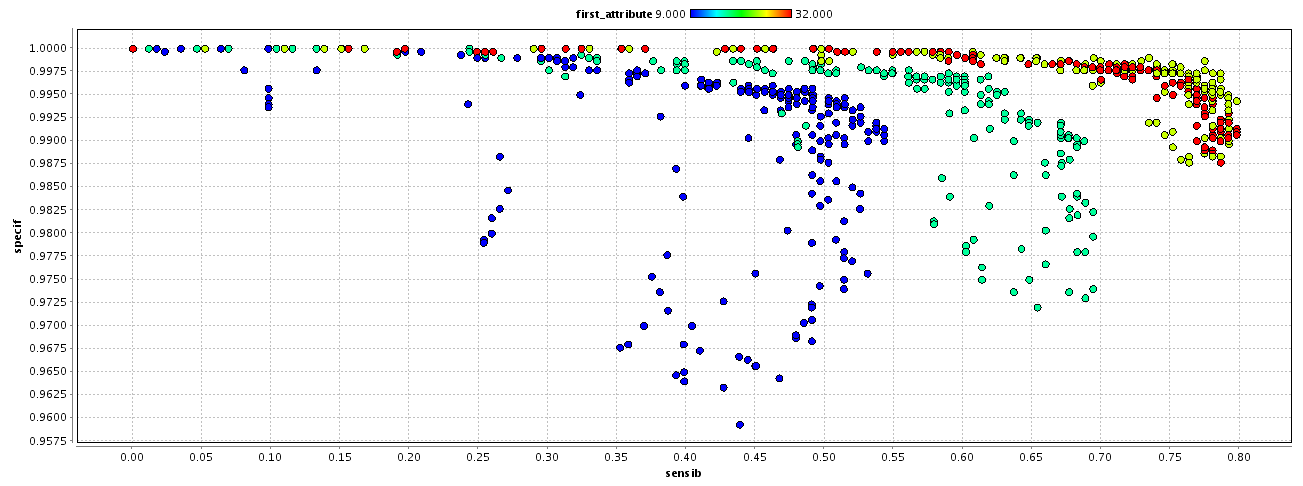
\includegraphics[width=14cm]{images/pareto_param_erosion.png}

{\small d) Base \'Erodée}


\end{center}
 \caption{Fronts de pareto des résultats de la recherche des meilleurs paramètres du classifieur (2/2). Pour chaque triplet de paramètres (C, $\gamma$, j), la sensibilité et la spécificité sont reportées sur le graphique. Le code couleur correspond à la valeur de j. En a) la base normalisation avec 200 points négatifs par image et une normalisation range. En b), la base érodée, avec 200 points négatifs par image et une normalisation mean, en b) la base enrichie avec 1000 points négatifs par image et une normalisation mean. }
\end{figure}




\begin{figure}[h!]
\label{fig:paramsParams}
%	\begin{center}
		\begin{tabular}{c c c c c c}
  \hline
  a	& Base Témoin 	& Base Erosion	& Base appauvrie& Base enrichie & Base normalisée \\
  \hline
 C 	& 464		& 74		& 5412		& 5412		& 10000 \\
\hline
$\gamma$& 0.0053	& 0.0094	& 0.00031	& 0.0017	& 0.052 \\
\hline
j	& 3		& 3		& 3		& 4		& 3	\\
\hline
\hline
Sensibilité& 0.75	& 0.80		& \textbf{0.82}		& 0.60		& 0.76	\\
\hline
Spécificité& 0.99	& 0.99		& 0.99		& 0.99		& 0.99 \\
\hline
Précision& 0.98		& 0.98		& 0.97		& 0.99		& 0.98 \\
\hline
 		\end{tabular}

%	\end{center}
\caption{Paramètres sélectionnés pour l'optimisation des performances. Sont indiqués pour chaque base le triplet de paramètres sélectionné ainsi que sa position sur le front de pareto.}
\end{figure}


\subsection{Base témoin}

Cette base contient des données normalisées par la méthode mean avec 200 points extraits de chaque image.

\subsubsection{Meilleurs paramètres de classification}

Les paramètres du classifieur sont déterminés par une recherche grille. La performance de chaque triplet (C, $\gamma$, j) est estimée en réalisant une cross-validation à 5 validations sur l'ensemble de la base d'apprentissage.
Les paramètres sont choisits à partir du front de pareto figure \ref{fig:paretoParams1}.a en maximisant la sensibilité.


\subsection{Base Erosion}

Cette base contient des données normalisées par la méthode mean/std avec 200 points extraits de chaque image érodée (2 voxels).

\subsubsection{Meilleurs paramètres}

Les paramètres sont choisits à partir du front de pareto figure \ref{fig:paretoParams1}.b en maximisant la sensibilité.


\subsection{Base Appauvrie}

Cette base contient des données normalisées par la méthode mean/std avec 100 points extraits de chaque image.

\subsubsection{Meilleurs paramètres}

Les paramètres sont choisits à partir du front de pareto figure \ref{fig:paretoParams2}.b en maximisant la sensibilité.




\subsection{Base Enrichie}

Cette base contient des données normalisées par la méthode mean/std avec 1000 points extraits de chaque image.

\subsubsection{Meilleurs paramètres}

Les paramètres sont choisits à partir du front de pareto figure \ref{fig:paretoParams2}.b en maximisant la sensibilité.





\subsection{Base Normalisation}

Cette base contient des données normalisées par la méthode range avec 200 points extraits de chaque image.

\subsubsection{Meilleurs paramètres}

Les paramètres sont choisits à partir du front de pareto figure \ref{fig:paretoParams2}.c en maximisant la sensibilité.



\subsection{Courbe Free-ROC}

Voir figure \ref{lab:froc_comp_static}
Le maximum de performances est apporté par la combinaison de 200 points avec mean/std.

\begin{figure}[h!]
 
 \begin{center}
   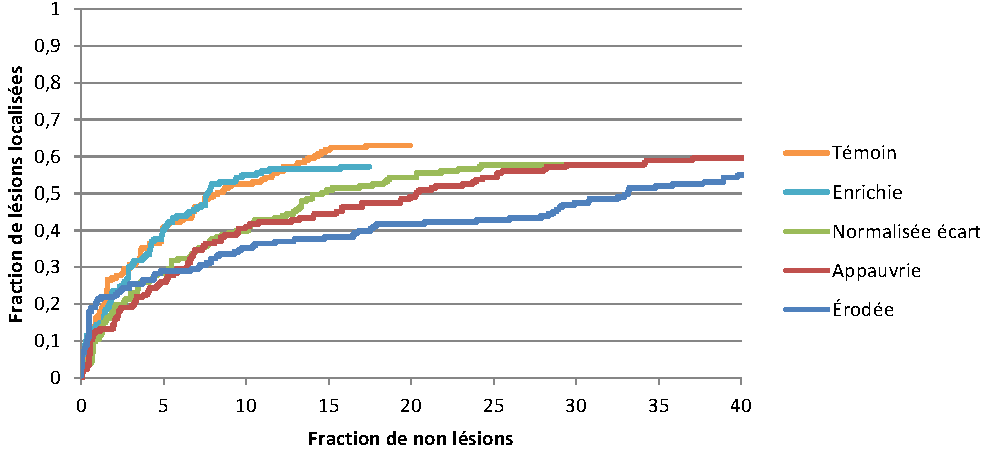
\includegraphics[width=15cm]{images/FROC_param}
 \end{center}
 \caption{\label{lab:froc_comp_static} Courbe Free-ROC comparant les performances du CAD sur une base témoin (normalisation moyenne et 200 points négatifs par image), sur une base enrichie (1000 points négatifs par image), sur une base appauvrie (100 points négatifs par image), sur une base normalisée différemment (normalisation entre -1 et +1 et 200 points négatifs par image) et enfin sur une base de 100 points négatifs par image mais dont les volumes ont été érodés de 2 voxels.}

\end{figure}


\subsection{Comparaison des performances JAFROC}

La p-value est de 0.049, ce qui permet pas déclarer que au moins deux paramètres testés sont différents. \ref{lab:fom_param}


\begin{figure}[h!]
 \begin{center}
   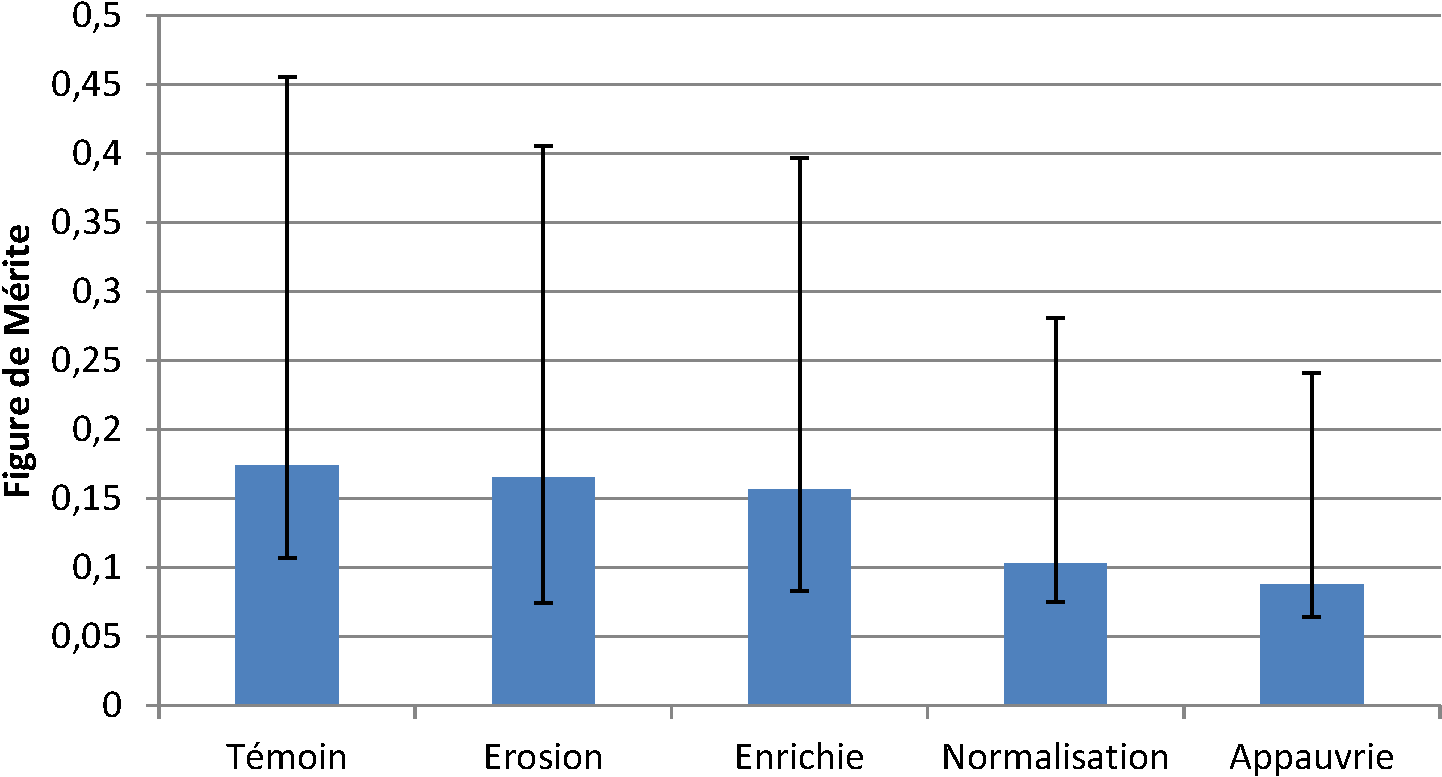
\includegraphics[width=15cm]{images/FOM_param}
 \end{center}
 \caption{ \label{lab:fom_param} Les FOM (Figure de Mérite) obetnues pour les différents paramètres}
\end{figure}

\FloatBarrier

\section{Comparaison des performances des différentes méthodes Poumon}

Les caractéristiques utilisées pour obtenir ces résultats sont les suivants :

\begin{itemize}
 \item 200 points tirés aléatoirement dans le volume de chaque image (hors tumeurs)
 \item normalisation par moyennage et neutralisation de la variance 
\end{itemize}


\begin{figure}[h!]

\begin{center}
 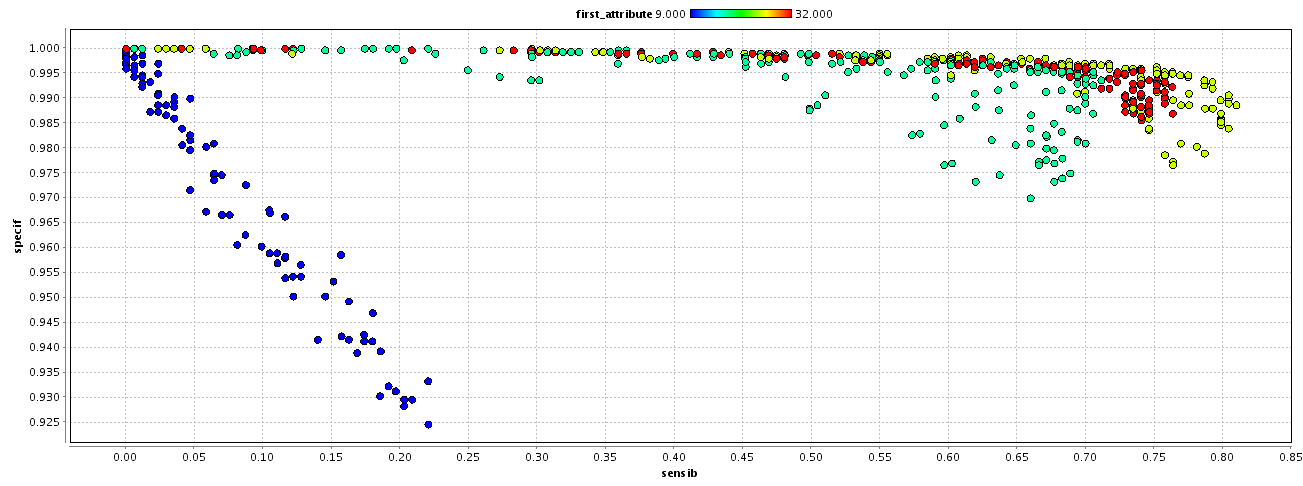
\includegraphics[width=14cm]{images/pareto_mod_IM.png}

{\small a) ET-IM}
\vspace{0.5cm}

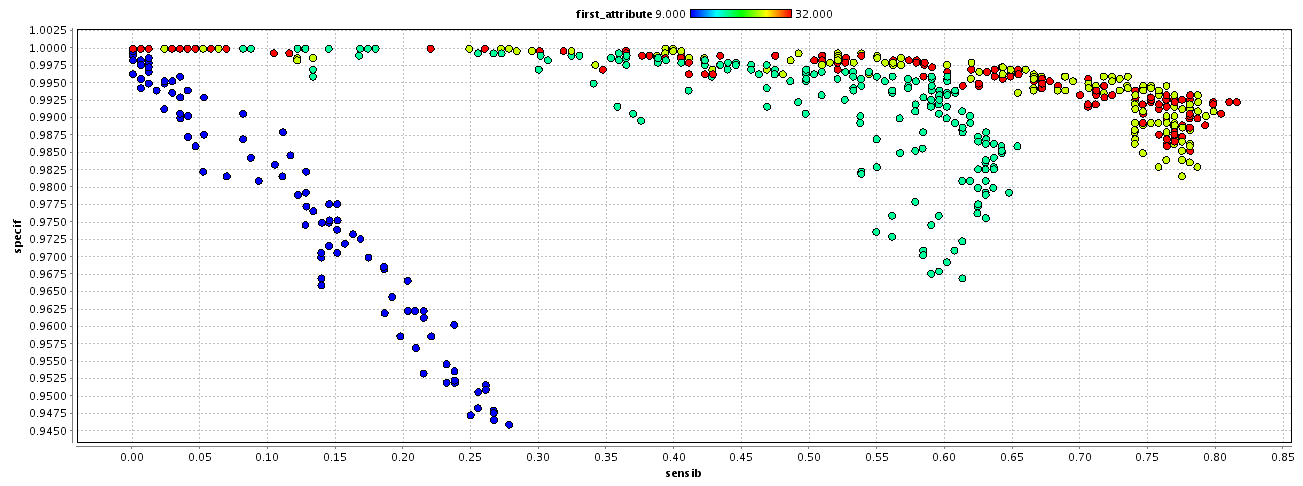
\includegraphics[width=14cm]{images/pareto_mod_LOR.png}
 
{\small b) ET-LOR}
\vspace{0.5cm}

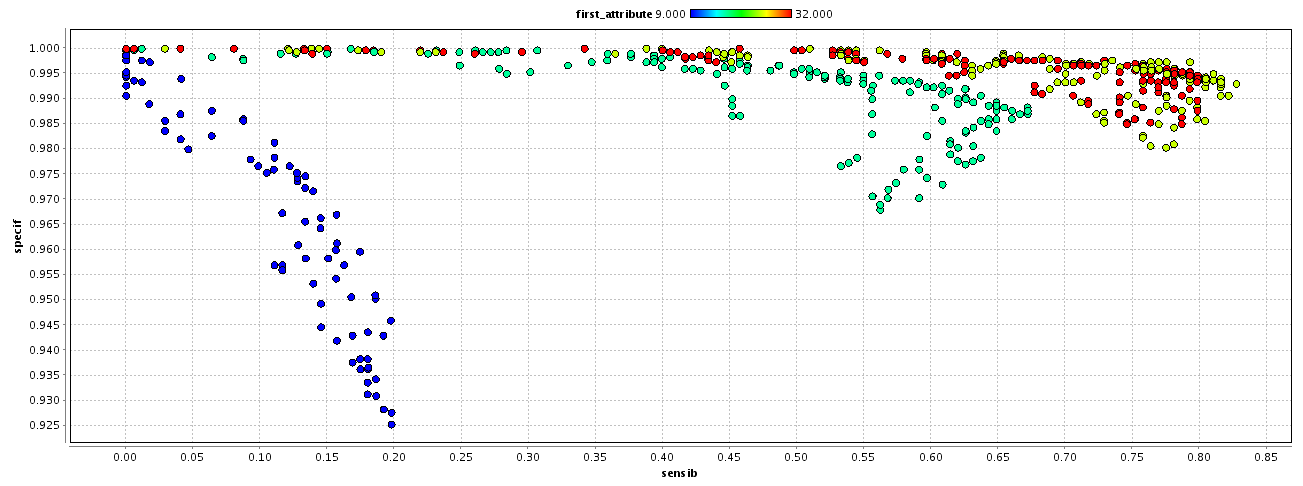
\includegraphics[width=14cm]{images/pareto_mod_NoCorr.png}

{\small c) ET-NoCorr}

\end{center}
 \caption{\label{fig:paretoModalite} Fronts de pareto des résultats de la rechdeche des meilleurs paramètres du classifieur pour les différentes modalitées, avec 200 points négatifs par image. Pour chaque triplet de paramètres (C, $\gamma$, j), la sensibilité et la spécificité sont reportées sur le graphique. Le code couleur correspond à la valeur de j. a) représente la correction d'image ET-IM, b) les images non corrigées du mouvement, et c) les images corrigées par ka méthode LOR.}
\end{figure}








\begin{figure}[h!]
\label{fig:paramsModPoumon}
%	\begin{center}
		\begin{tabular}{c| c c c c c}
  \hline
  a	& Base Statique	& Base IM	& Base LOR	& Base NoCorr	\\
  \hline
 C 	& 464		& 10000		& 10000		& 10000		\\
\hline
$\gamma$& 0.0053	& 0.00097	& 0.00031	& 0.00055	\\
\hline
j	& 3		& 3		& 4		& 3		\\
\hline
\hline
Sensibilité& 0.75	& 0.81		& 0.82		& 0.83	\\
\hline
Spécificité& 0.99	& 0.99		& 0.99		& 0.99		\\
\hline
Précision& 0.98		& 0.98		& 0.98		& 0.98		\\
\hline
 		\end{tabular}

%	\end{center}
\caption{Paramètres sélectionnés pour l'optimisation des performances du Poumon. Sont indiqués pour chaque base le triplet de paramètres sélectionné ainsi que sa position sur le front de pareto.}
\end{figure}



\subsection{ET-IM}

Cette base contient des données normalisées par la méthode mean/std. avec 200 points extraits de chaque image.

\subsubsection{Front de pareto}

Les paramètres sont choisits à partir du front de pareto figure \ref{fig:paretoModalite}.a en maximisant la sensibilité.

\subsubsection{Meilleurs paramètres}

Choisit en maximisant la sensibilité.			

Voir \ref{fig:paramsModPoumon}


\subsection{ET-LOR}

Cette base contient des données normalisées par la méthode mean/std. avec 200 points extraits de chaque image.

\subsubsection{Front de pareto}

Les paramètres sont choisits à partir du front de pareto figure \ref{fig:paretoModalite}.b en maximisant la sensibilité.


\subsubsection{Meilleurs paramètres}

Choisit en maximisant la sensibilité.

Voir \ref{fig:paramsModPoumon}

\subsection{ET-NoCorr}

Cette base contient des données normalisées par la méthode mean/std. avec 200 points extraits de chaque image.

\subsubsection{Front de pareto}

Les paramètres sont choisits à partir du front de pareto figure \ref{fig:paretoModalite}.c en maximisant la sensibilité.

\subsubsection{Meilleurs paramètres}

Voir \ref{fig:paramsModPoumon}

\subsection{Comparaison des performances JAFROC}

La p-value est de 0.10, ce qui ne permet pas de déclarer que statistiquement les données sont différentes : \ref{lab:fom_mod19}.

\begin{figure}[h!]
 \begin{center}
   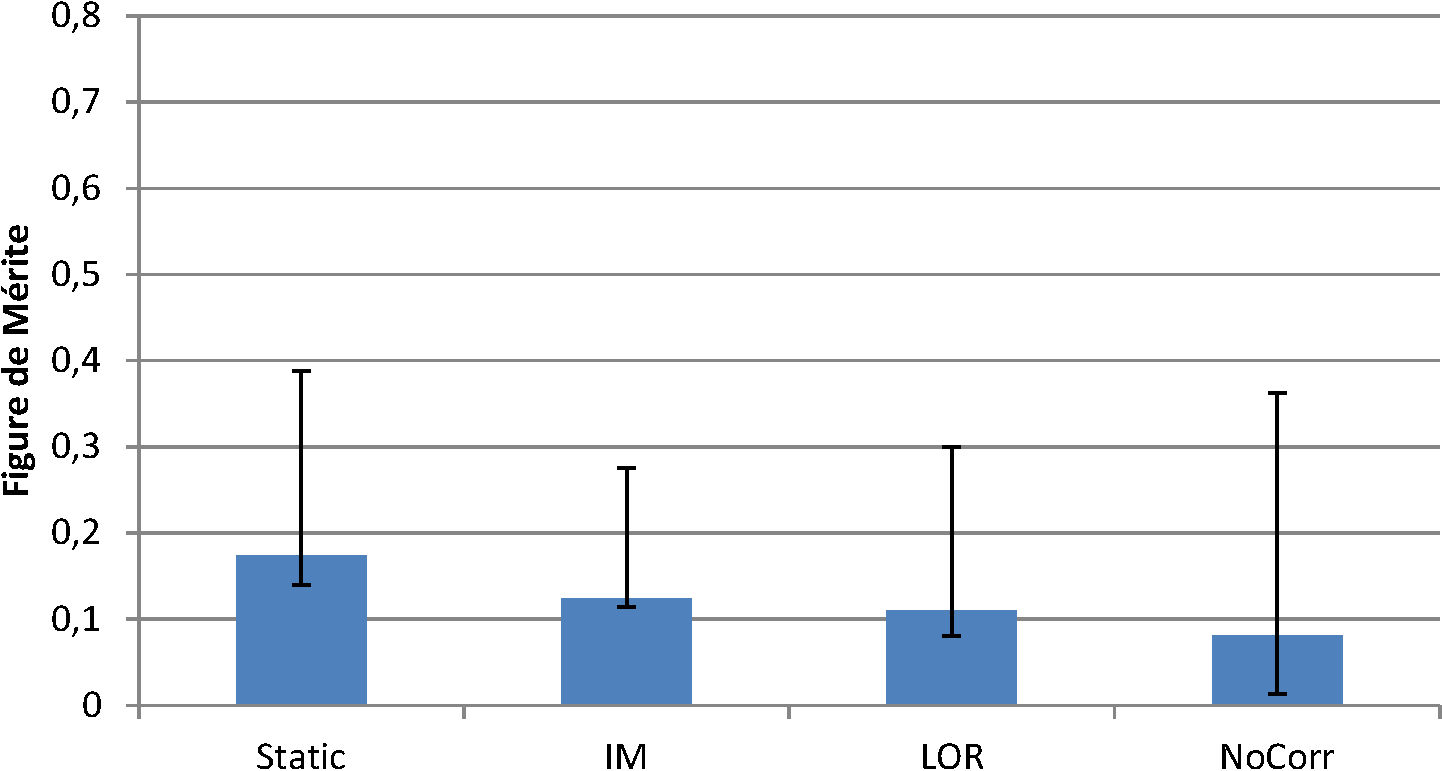
\includegraphics[width=15cm]{images/FOM_mod}
 \end{center}
 \caption{ \label{lab:fom_mod19} Les FOM (Figure de Mérite) obetnues pour les différentes modalités.}
\end{figure}

\subsection{Courbes Free-ROC}

Voir figure \ref{lab:froc_mod}.
Le maximum de performances est apporté par les images statiques, suivi par les images ET-IM.

\begin{figure}[h!]
 \begin{center}
   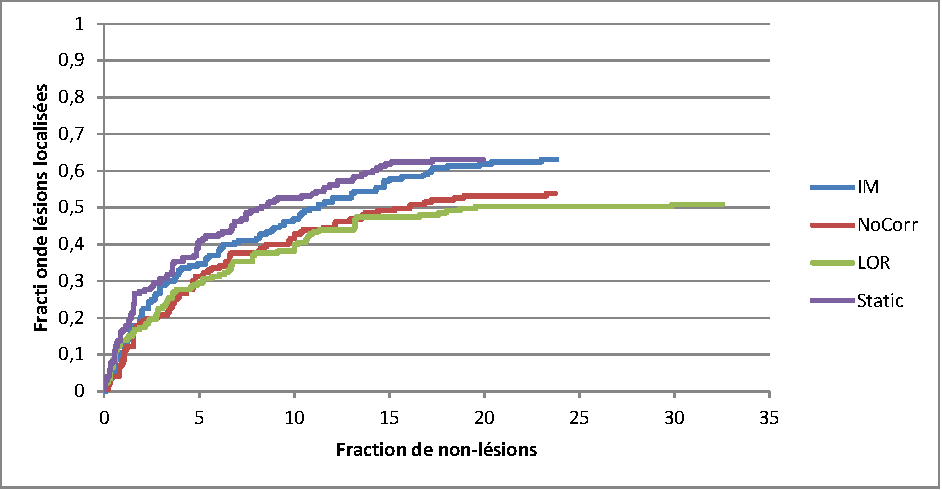
\includegraphics[width=15cm]{images/FROC_mod}
 \end{center}
 \caption{ \label{lab:froc_mod} Courbe Free-ROC comparant les performances du CAD selon les modalités de correction du mouvement respiratoire.}
\end{figure}








\FloatBarrier

\section{Comparaison des performances des différentes méthodes Foie}

Les caractéristiques utilisées pour obtenir ces résultats sont les suivants :

\begin{itemize}
 \item 200 points tirés aléatoirement dans le volume de chaque image (hors tumeurs)
 \item normalisation par moyennage et neutralisation de la variance 
\end{itemize}

\subsection{Comparaison des performances JAFROC}

La p-value est de 0.1, ce qui ne permet pas de déclarer que statistiquement les données sont différentes : \ref{lab:fom_mod19}


\begin{figure}[h!]
 \begin{center}
   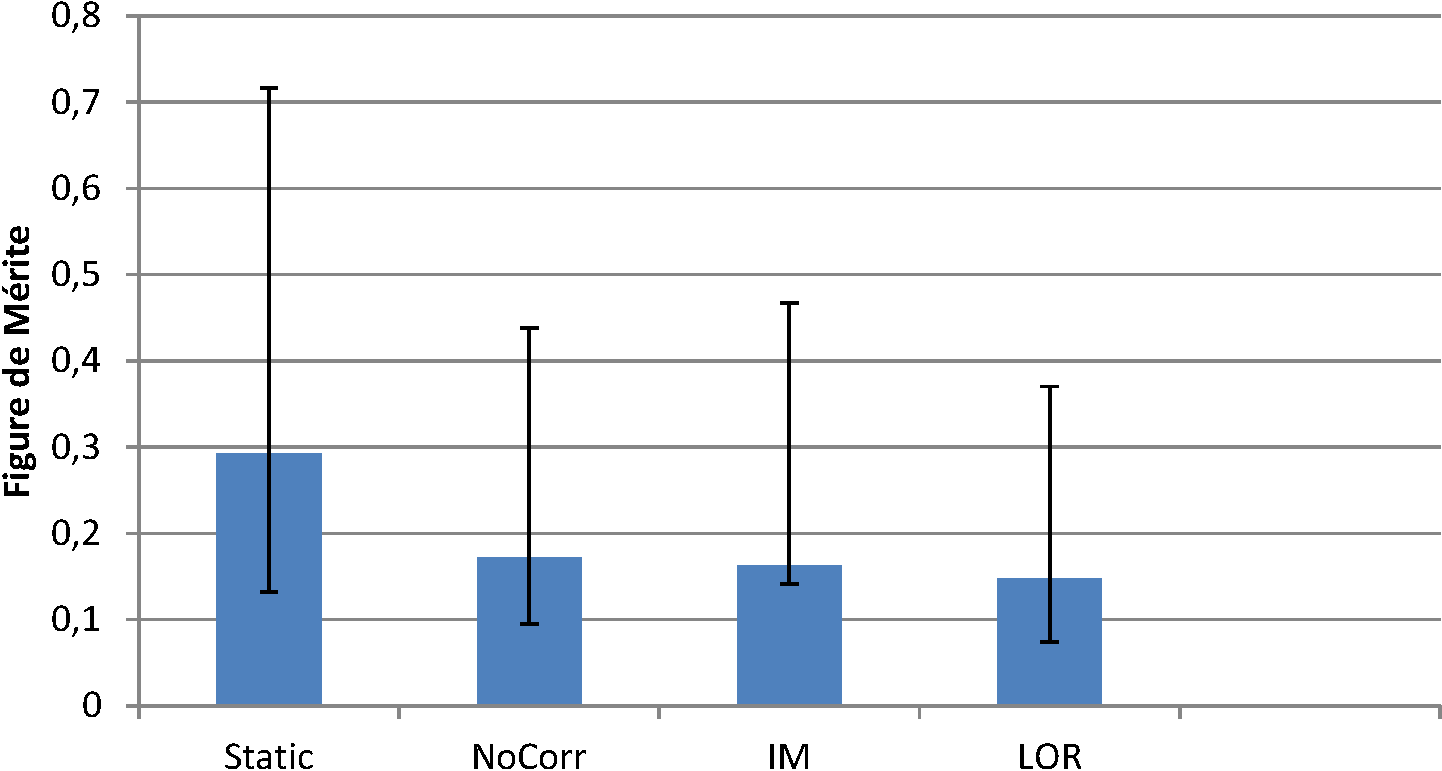
\includegraphics[width=15cm]{images/FOM_mod19}
 \end{center}
 \caption{ \label{lab:fom_mod19} Les FOM (Figure de Mérite) obetnues pour les différentes modalités.}
\end{figure}


\subsection{Courbes Free-ROC}

Voir figure \ref{lab:froc_mod19}.
Le maximum de performances est apporté par les images statiques, suivi par les images ET-IM.

\begin{figure}[h!]
 \begin{center}
   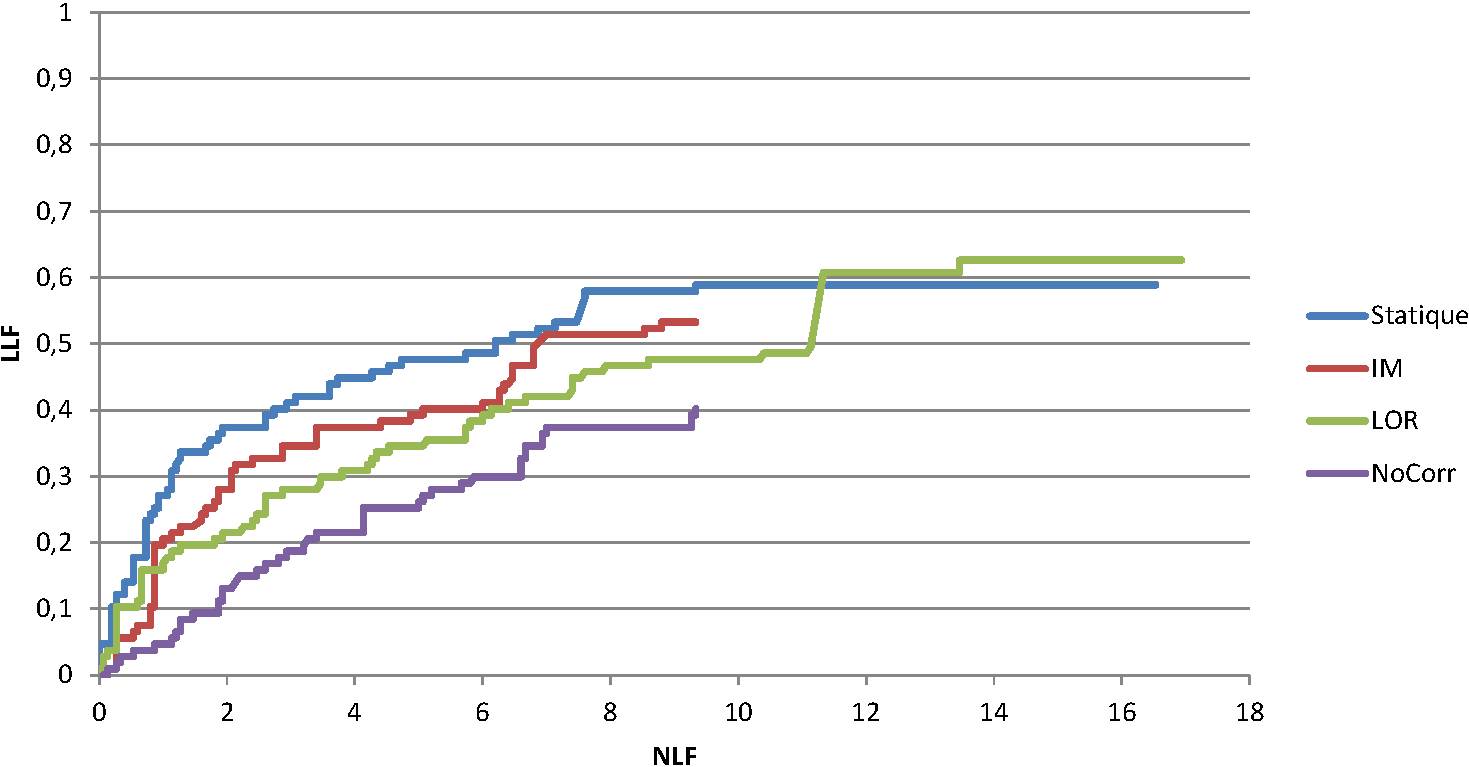
\includegraphics[width=15cm]{images/FROC_mod19}
 \end{center}
 \caption{ \label{lab:froc_mod19} Courbe Free-ROC comparant les performances du CAD selon les modalités de correction du mouvement respiratoire.}
\end{figure}


\begin{figure}[h!]

\begin{center}
 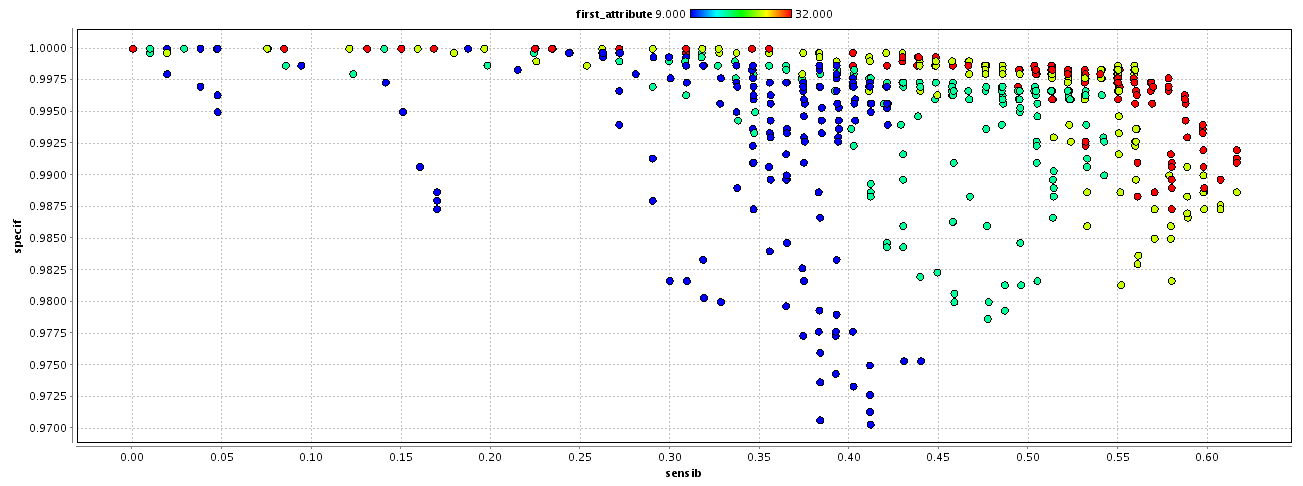
\includegraphics[width=14cm]{images/pareto_mod_Static19.png}

{\small a) ET-Static}
\vspace{0.5cm}

 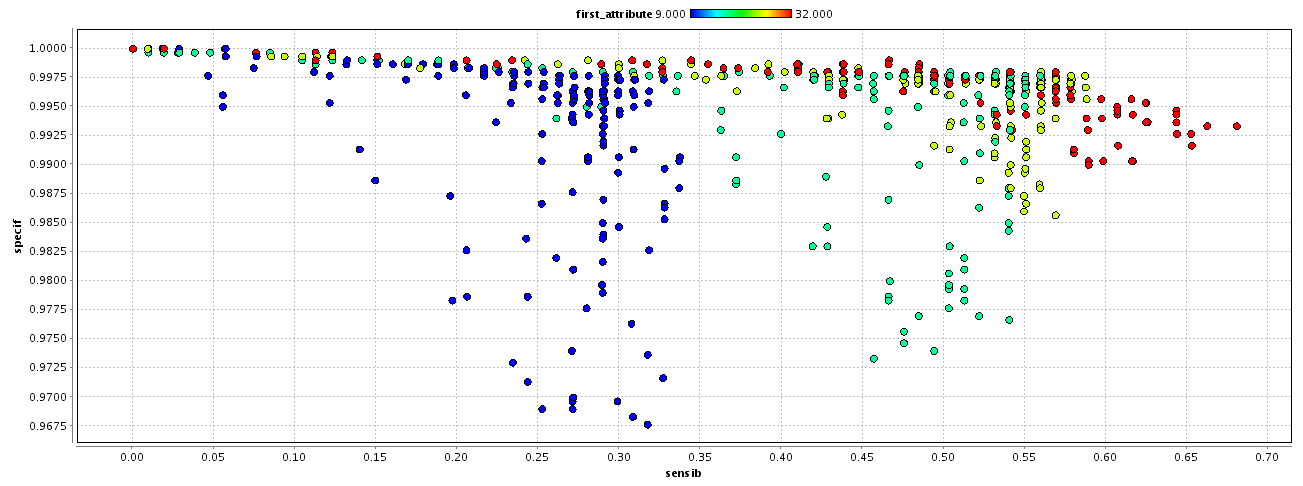
\includegraphics[width=14cm]{images/pareto_mod_IM19.png}

{\small b) ET-IM}

\end{center}
 \caption{\label{fig:paretoModalite19_1} Fronts de pareto des résultats de la rechdeche des meilleurs paramètres du classifieur pour les différentes modalitées, avec 200 points négatifs par image. Pour chaque triplet de paramètres (C, $\gamma$, j), la sensibilité et la spécificité sont reportées sur le graphique. Le code couleur correspond à la valeur de j. a) représente la correction d'image ET-Static, b) les images corrigées du mouvement post-reconstruction.}
\end{figure}

\begin{figure}[h!]

\begin{center}
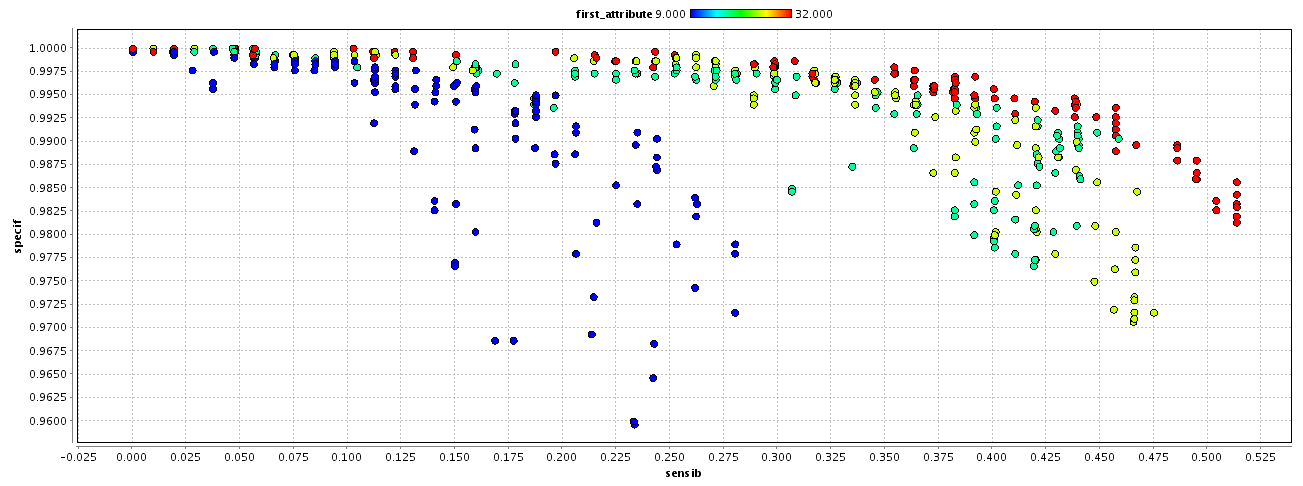
\includegraphics[width=14cm]{images/pareto_mod_LOR19.png}
 
{\small c) ET-LOR}
\vspace{0.5cm}

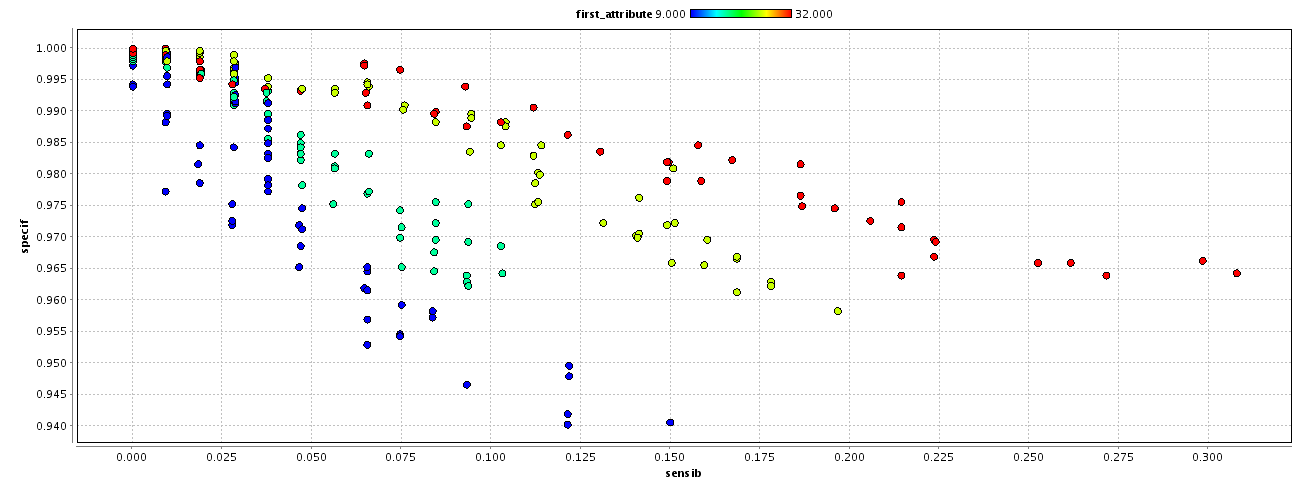
\includegraphics[width=14cm]{images/pareto_mod_NoCorr19.png}

{\small d) ET-NoCorr}

\end{center}
 \caption{\label{fig:paretoModalite19_2} Fronts de pareto des résultats de la rechdeche des meilleurs paramètres du classifieur pour les différentes modalitées, avec 200 points négatifs par image. Pour chaque triplet de paramètres (C, $\gamma$, j), la sensibilité et la spécificité sont reportées sur le graphique. Le code couleur correspond à la valeur de j. c) représente la correction d'image pendant la reconstruction et d) le images non corrigées.}
\end{figure}



% Static : 857.6958985908936	0.001709975946676697	32.0	0.9790779315594078	0.6160173160173159	0.992
% LOR	 : 251.18864315095797	0.005323362023203629	32.0	0.969422309209811	0.5134199134199134	0.9856666666666667 
% NoCorr : 5411.6952654646375	0.001709975946676697	32.0	0.9417478291936561	0.30779220779220784	0.9643333333333333
% IM	 : 5411.6952654646375	5.49280271653059E-4	32.0	0.9826195691007659	0.6805194805194804	0.9933333333333334
\begin{figure}[h!]
\label{fig:paramsModFoie}
%	\begin{center}
		\begin{tabular}{c| c c c c c}
  \hline
  a	& Base Statique	& Base IM	& Base LOR	& Base NoCorr	\\
  \hline
 C 	& 858		& 5412		& 251		& 5412		\\
\hline
$\gamma$& 0.002		& 0.00055	& 0.0053	& 0.0017	\\
\hline
j	& 4		& 4		& 4		& 4		\\
\hline
\hline
Sensibilité& 0.62	& 0.68		& 0.51		& 0.31	\\
\hline
Spécificité& 0.99	& 0.99		& 0.99		& 0.96		\\
\hline
Précision& 0.98		& 0.98		& 0.97		& 0.94		\\
\hline
 		\end{tabular}

%	\end{center}
\caption{Paramètres sélectionnés pour l'optimisation des performances du Foie. Sont indiqués pour chaque base le triplet de paramètres sélectionné ainsi que sa position sur le front de pareto.}
\end{figure}
% 
% Tests en prenant en compte le bord du poumon (sans faire l'érosion de 2 voxels) avec 200 ou 1000 points négatifs par image. Paramètres de SVM par défaut (g=0.001, C=100), images statiques.
% Cette fois-ci, étant donné le faible nombre de FP, j'ai préféré afficher les performances MAXIMALES obtenues.
% 
% Entre parenthèse un seuil alternatif pour pouvoir comparer les performances à NLF comparables.
% 
% \begin{tabular}{|c|c|c|c|c|c|c|}
%  \hline
% 				& \multicolumn{3}{|c|}{Réduction Simple}& \multicolumn{3}{|c|}{Réduction Étendue} \\
%  \hline
%  PNI	& Seuil	& LLF	& NLF	 		& Seuil		& LLF	& NLF	\\
%  \hline
% 1000 				&-1.05	& 86	& 20.47 	 	& -1.078	& 84	& 15.8	\\
%  \hline
% 200 				& -0.77	(-0.68)& 92 (86)& 26.4 (21.7)	& -0.679 & 84 & 15.7\\
%  \hline
% 
% \end{tabular}
% 
% 
% \subsubsection{Choix de Normalisation}
% 
% Test avec 15000 Points négatifs, images statiques
% 
% Front de pareto indiquant les performances atteintes (sensib et specif) selon les niveaux de décomposition :
% 
% 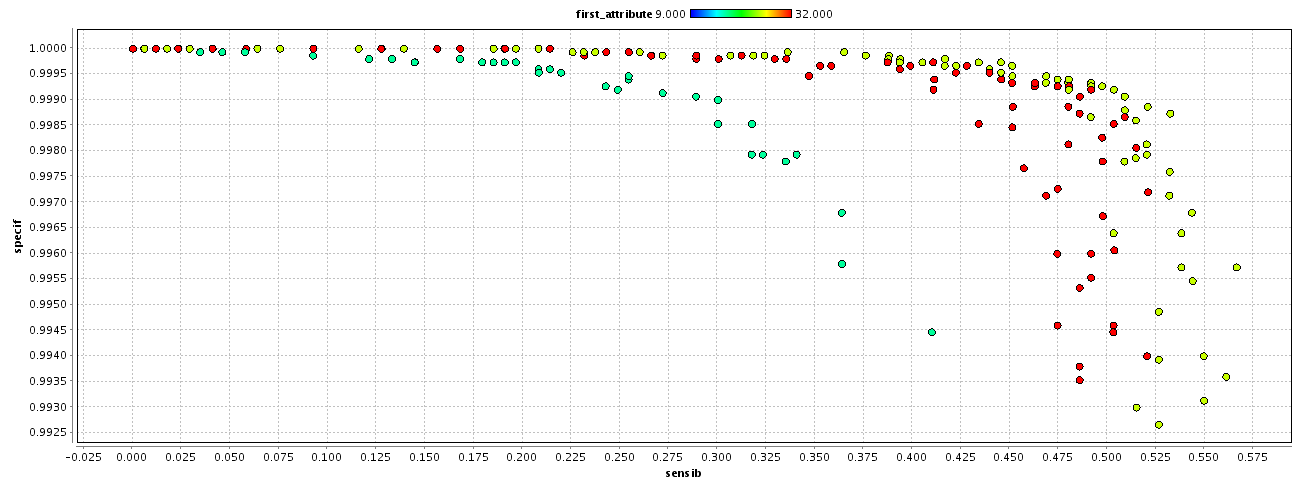
\includegraphics[width=14cm]{images/paretoNorm.png}
% 
% Il a été choisit le point haut droit de coordonnées suivantes : 
% 
% 
% \begin{itemize}
% \item C = 10000.0
% \item gamma = 0.016572270086699932
% \item j = 3
% \end{itemize}
% 
% Résultats :
% \begin{itemize}
% \item Sensib : 0.993
% \item Specif : 0.532
% \item Accuracy : 0.999
% \end{itemize}
% 
% 
% 
% \section{Comparaison des performances Free-ROC}
% 
% \subsection{Influence des paramètres de l'observateur}
% 
% La courbe Free-ROC \ref{fig:JAFROC_Compare_Static} suivante
% 
% \begin{figure}[h!]
% 	\vspace{-0.5cm}	
% 	\begin{center}
% 		\begin{tabular}{c c}
% 			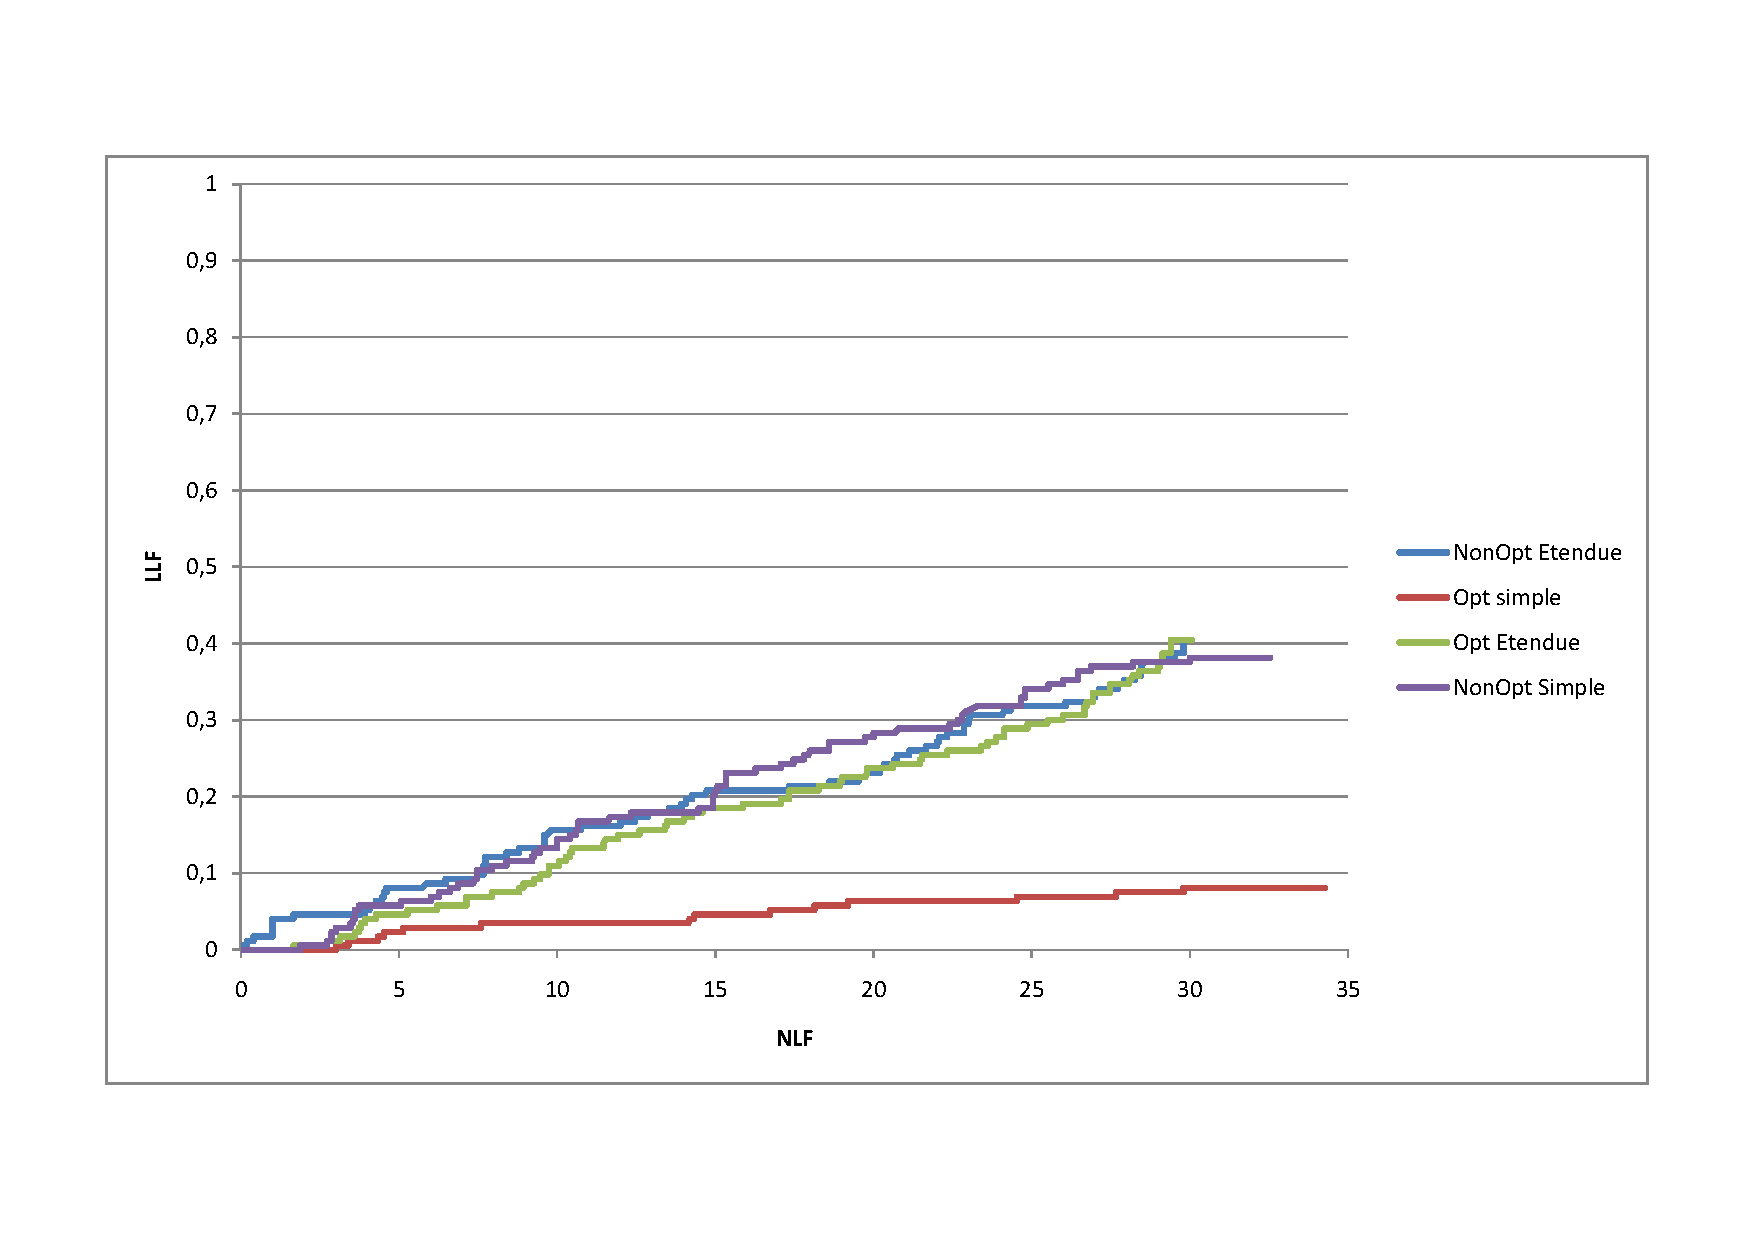
\includegraphics[width=14cm]{images/JAFROC_Compare_Static}
% 		\end{tabular}
% 	\end{center}
% 	\vspace{-1cm}
% 	\caption{Comparaison des performances du système CAD selon que le classifieur est optimisé (Opt) ou non optimisé (NonOpt) et que l'on utilise le système de réductions de faux positifs simple ou étendu. Réalisé sur des données statiques.}
% 	\label{fig:JAFROC_Compare_Static}
% \end{figure}